\documentclass[tikz,border=10pt]{standalone}
\begin{document}
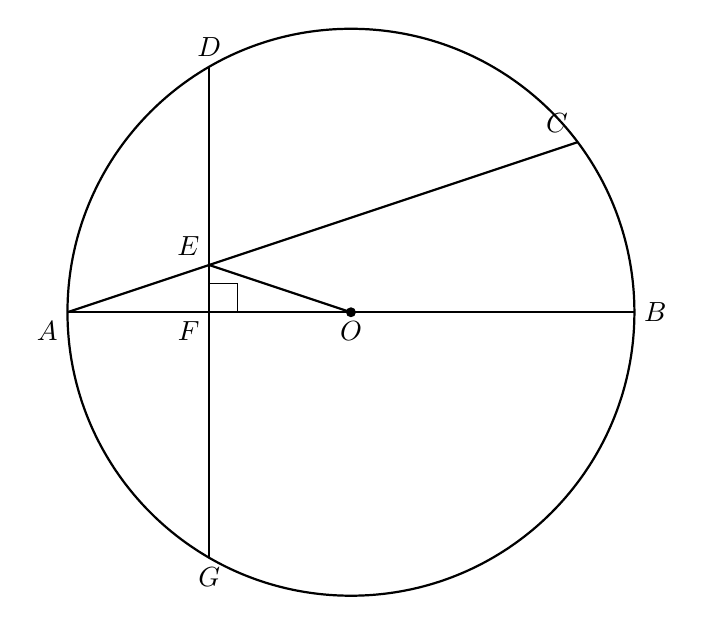
\begin{tikzpicture}[scale=1.2]
\coordinate (O) at (0,0);
\coordinate (A) at (-3,0);
\coordinate (B) at (3,0);
\coordinate (D) at (-1.5,2.598);
\coordinate (G) at (-1.5,-2.598);
\coordinate (F) at (-1.5,0);
\coordinate (E) at (-1.5,0.5);
\coordinate (C) at (2.4,1.8);

\draw[thick] (O) circle (3);
\draw[thick] (A) -- (B);
\draw[thick] (D) -- (G);
\draw[thick] (A) -- (C);
\draw[thick] (E) -- (O);
\draw (-1.5,0) -- (-1.2,0) -- (-1.2,0.3) -- (-1.5,0.3) -- cycle;

\fill (O) circle (1.5pt);

\node[below left] at (A) {$A$};
\node[right] at (B) {$B$};
\node[above] at (D) {$D$};
\node[below] at (G) {$G$};
\node[above left] at (C) {$C$};
\node[below left] at (F) {$F$};
\node[above left] at (E) {$E$};
\node[below] at (O) {$O$};
\end{tikzpicture}
\end{document}
